% !TeX root = ../dd.tex

\section{Implemention, Integration and Test Plan}
% Identify here the order in which you plan
% to implement the subcomponents of your system and the order in which you plan % to integrate such subcomponents and test the integration.

\subsection{Overview}

The application is composed of three decoupled layers (\emph{client}, \emph{business}, and \emph{data}) which can be developed and unit tested independendly, and integration tested at the end.

\paragraph{Front-end components} They consist of the mobile and web application, that have been presented in Chapter \ref{ch:2}. They consist mostly of presentational components that belong to the client layer. Since both applications rely on a REST API, and should likely reuse portions of the codebase, they can be easily unit tested by mocking of the REST API.

\paragraph{Back-end components} They're components that resides in the server, from both the business and the data layer.

\paragraph{External components} They consist of the \emph{Maps API}, the \emph{SMS API}, and the \emph{Notification API}. Since they're provided by third parties, they're supposed to be reliable and conform to their specifications.

\subsection{Feature identification}

To better plan the testing each component will require, it's useful to visualize them in a table (Table \ref{tab:features}) where each components is associated with its difficulty of implementation and its importance for the system.

% TODO TABLE
\begin{table}[h]
    \centering
    \begin{tabular}[h]{|l|l|l|}
        \hline
        \textbf{Feature} & \textbf{Importance} & \textbf{Difficulty} \\\hline
        User login & High & Medium \\
        Join queue & High & Medium \\
        Reserve timeslot & High & High \\
        Search store & Medium & Medium \\
        View store details & Medium & Low \\
        Notify customers & High & Medium \\
        Adjust store parameters (managers) & High & Medium \\
        Add/Remove/Edit stores (managers) & Medium & Low \\
        View statistics (managers) & Low & Low \\
        \hline
    \end{tabular}
    \caption{Importance and difficulty of required features}
    \label{tab:features}
\end{table}

\subsection{Approach}

All components will be implemented and tested with a \emph{bottom-up} approach, in order to reduce the overhead that would have derived from a \emph{top-down} one.

Components from the same subsystem (for example, the backend) can be implemented, unit-tested and integration-tested without a real need of components from another subsystem. This allows developers to develop in parallel the client and the backend, thus speeding up the development process.

Finally, after the final integration testing is complete, it's important to verify the adherence to the specified requirements.

In particular, the web and mobile application can be developed without need for a server, as the REST API can be easily mocked in tests.

\subsection{Components integration}

Here components and subsystems are illustrated via graphs where the arrow $x \longrightarrow y$ means ``$x$ depends on $y$''. Subsystems are a group of components meant to be integration tested together after unit testing.

%%% 1
The first components to be tested together are the \emph{Query Manager} and the \emph{DBMS}, because it serves as the foundation upon all the other components rely when handling data.

\begin{figure}[H]
    \centering
    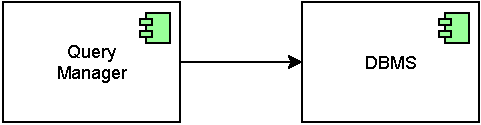
\includegraphics[height=5em]{images/draw.io/data_subsystem.pdf}
    \caption{Data subsystem}
    \label{fig:data_subsystem}
\end{figure}

%%% 2
The following three subsystems might be developed in any order, or simultaneously, as they do not depend on each other.

It is recommended to develop the \emph{Store Handler Subsystem} first, as it represent the core functionality of the product. This is the item that should be the most carefully tested. It also requires the \emph{Notification Manager} component to be implemented during integration testing.

\begin{figure}[H]
    \centering
    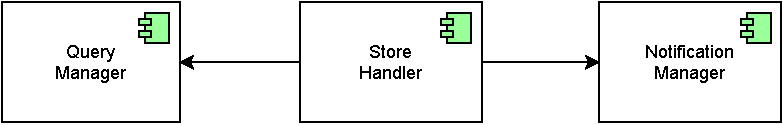
\includegraphics[height=5em]{images/draw.io/store_handler_subsystem.pdf}
    \caption{Store handler subsystem}
    \label{fig:store_handler_subsystem}
\end{figure}

The \emph{Account Subsystem} is critical because it's needed to regulate the use of the product through the creation of the account. It should be tested with particular attention to user's input, handling invalid data correctly.

\begin{figure}[H]
    \centering
    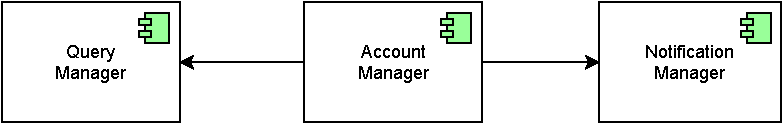
\includegraphics[height=5em]{images/draw.io/account_subsystem.pdf}
    \caption{Account subsystem}
    \label{fig:account_subsystem}
\end{figure}

The \emph{Store Search Subsystem} is the least critical subsystem to be implemented, and it doesn't rely on any other component beside the \emph{Query Manager}.

\begin{figure}[H]
    \centering
    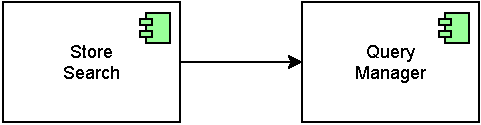
\includegraphics[height=5em]{images/draw.io/store_search_subsystem.pdf}
    \caption{Store search subsystem}
    \label{fig:store_search_subsystem}
\end{figure}

%%% 3

Once the critical subsystems have been implemented, it's the right time to implement and test the \emph{Admin Services Subsystem}, which is the backend for all operations performable by store managers. It's important to test that all formal requirements are satisfied and cannot be violated by the user.
\begin{figure}[H]
    \centering
    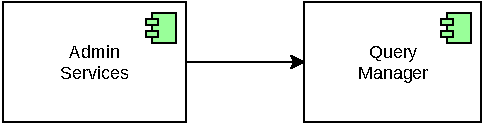
\includegraphics[height=5em]{images/draw.io/admin_services_subsystem.pdf}
    \caption{Admin services subsystem}
    \label{fig:admin_services_subsystem}
\end{figure}

%%% 4
At this point all subsystems have been implemented and tested, so the next step is performing integration tests between the client (front-end) and the server (back-end).

The client web and mobile app needs to interface with both the \emph{Store Handler Subsystem} and the \emph{Store Search Subsystem}.

\begin{figure}[H]
    \centering
    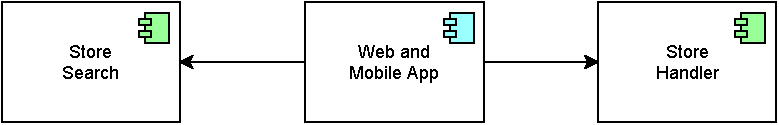
\includegraphics[height=5em]{images/draw.io/web_mobile_app_integration.pdf}
    \caption{Client application integration}
    \label{fig:client_application_integration}
\end{figure}

The totem needs to interface only with the \emph{Store Handler Subsystem}, since the store it's predetermined at deployment.

\begin{figure}[H]
    \centering
    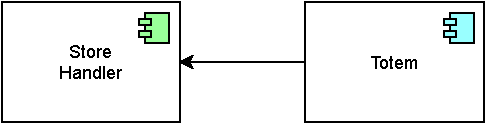
\includegraphics[height=5em]{images/draw.io/totem_integration.pdf}
    \caption{Totem integration}
    \label{fig:totem_integration}
\end{figure}

The \emph{Admin Control Panel} has its own interface that should be tested.

\begin{figure}[H]
    \centering
    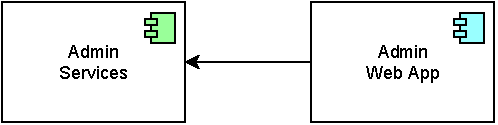
\includegraphics[height=5em]{images/draw.io/admin_panel_integration.pdf}
    \caption{Admin panel integration}
    \label{fig:admin_panel_integration}
\end{figure}

%%% full
The final result of integration of front-end, back-end and external components is the following:
\begin{figure}[H]
    \centering
    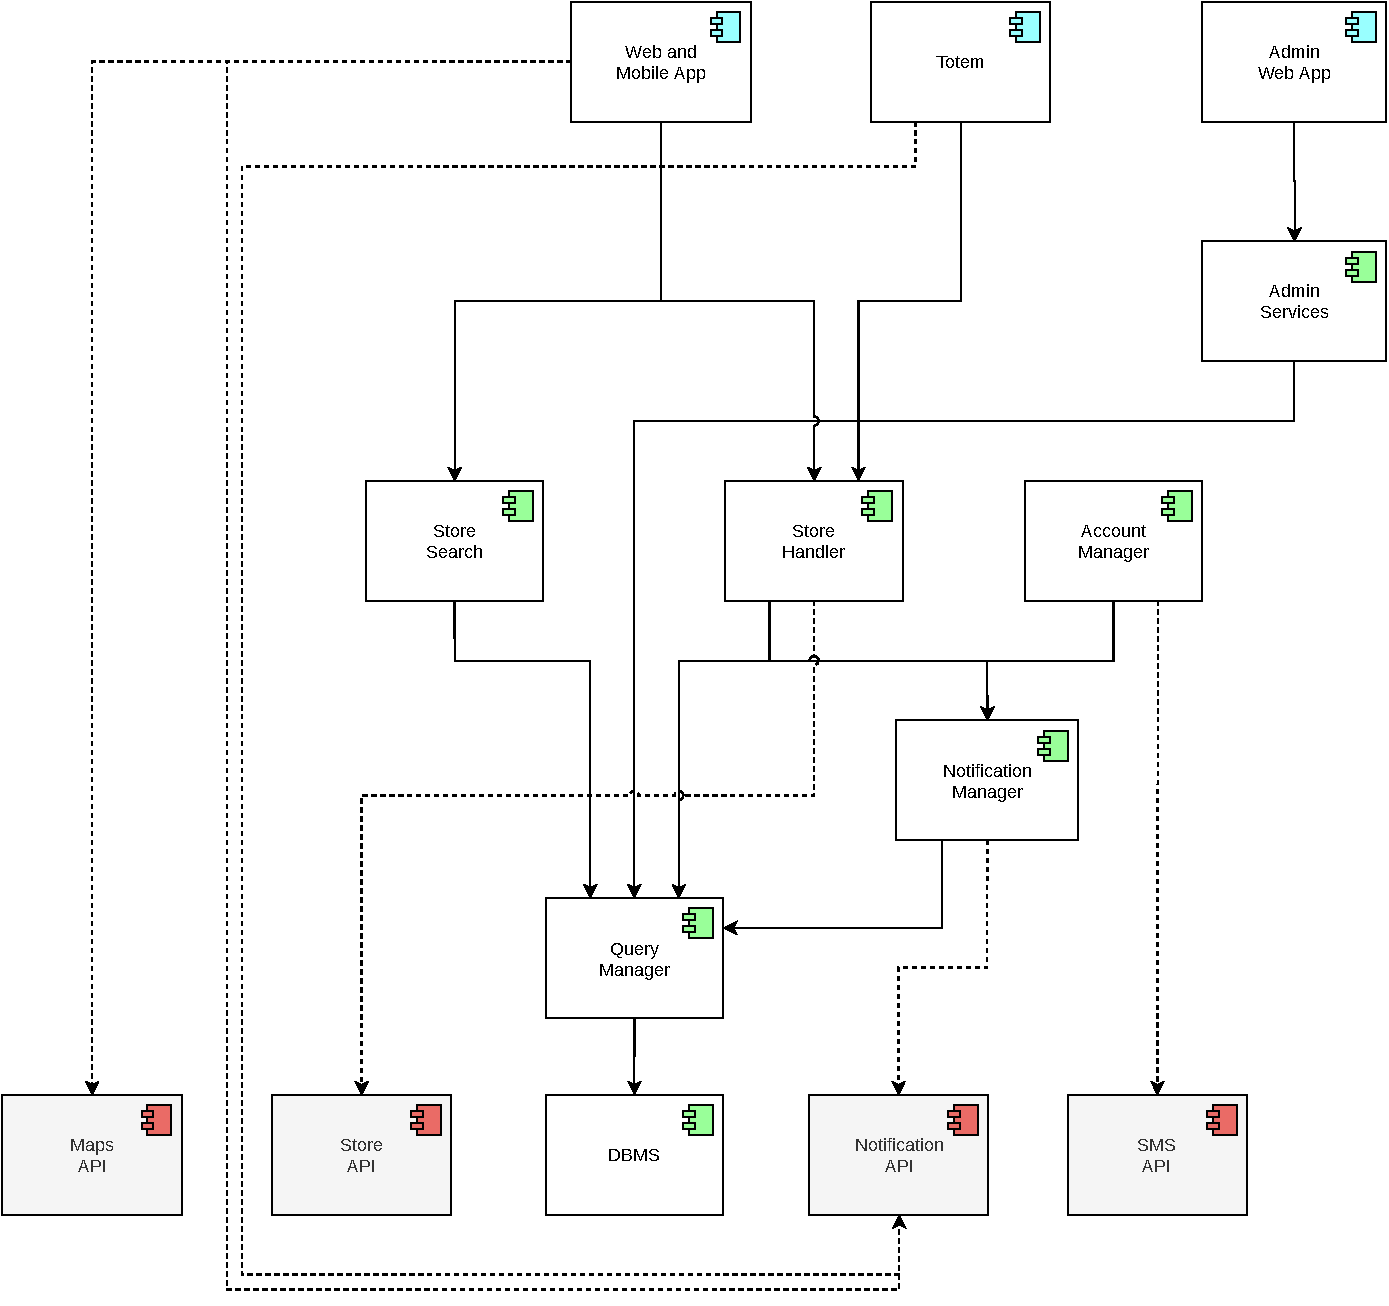
\includegraphics[width=0.8\linewidth]{images/draw.io/integration_full.pdf}
    \caption{Full component and subsystems integration.\\ A dashed line means integration testing with external components/APIs.}
    \label{fig:full_components_integration}
\end{figure}